\documentclass[]{article}

\usepackage{marginnote}
\usepackage{verbatim}
\usepackage[letterpaper,left=3cm,right=4cm]{geometry}

\usepackage{graphicx}

\usepackage{fancyhdr}
\pagestyle{fancy}

\usepackage[colorlinks=true]{hyperref}
\hypersetup{allcolors={blue}}
\hypersetup{pdftitle={Probability Distribution Workshop}}
\hypersetup{pdfauthor={Paul Glezen}}
\hypersetup{pdfcreator={Latex}}
\hypersetup{pdfkeywords={ISAB, Workshop, Probability, Distributions}}

\setlength{\parindent}{0em}
\setlength{\parskip}{1em}

\title{Probability Distribution Workshop}
\author{Los Angeles County\\ISAB}
\date{}

\begin{document}
\maketitle

\section{Introduction}

This workshop is a review of common probability distributions.
It has two principal goals.

\begin{enumerate}

\item Serve as a review for people that have not studied this material
   for a while.

\item Provide exercise for people to familiarize themselves with their
   Python and R distributions.

\end{enumerate}

The exercises themselves are detailed in \emph{Jupyter notebooks} for 
Python and \emph{R markdown} for R.  This mathematical supplement
serves to provide some theoretical motivation for functions encountered
in the Python and R libraries.

\subsection{Availability}

The source code for this document
along with the Python and R exercises are available from the ISAB
GitHub repository.

\href{https://github.com/lacounty-isab/workshops/tree/master/distributions}{https://github.com/lacounty-isab/workshops/tree/master/distributions}

\subsection{Who are We?}

ISAB (Information Systems Advisory Body) is a subcommittee of the 
CCJCC (Countywide Criminal Justice Coordination Committee)
of Los Angeles County, California.
ISAB is a multi-jurisdictional organization serving the justice
communities within the county. 
The ISAB Data Science Committee (IDSC) addresses data science issues
faced by the community. This article addresses skill development.
It is not intended as an endorsement of any one product
or technology.

More details on ISAB and CCJCC can be found on their websites.

\begin{itemize}
\item[ISAB] \href{http://ccjcc.lacounty.gov/Subcommittees-Task-Forces/Information-Systems-Advisory-Board-ISAB}{http://ccjcc.lacounty.gov/Subcommittees-Task-Forces/Information-Systems-Advisory-Board-ISAB}
\item[CCJCC] \href{http://ccjcc.lacounty.gov/}{http://ccjcc.lacounty.gov/}
\end{itemize}

\section*{Random Variables}

Since this article is not intended to be a foundational exposition on
probability theory, we'll jump right in with a review of random variables.
Recall that an event space $\Omega$ is a set of possible outcomes for an
experiment.  In the case of flipping a single coin, we would have

$$
\Omega = \{\mbox{heads}, \mbox{tails}\}
$$

A random variable $X$ is an assignment from the event space to the real
numbers.

$$
X: \Omega \rightarrow {\rm I\!R}
$$

An example for the case of a coin flip might be

\begin{eqnarray*}
X(\mbox{tails}) & = & 0\\
X(\mbox{heads}) & = & 1
\end{eqnarray*}

A less trivial example would be flipping a coin 100 times where
the outcome is the number of heads.  There are many random varialbes
you could define on this event space.

\begin{itemize}
\item the number of heads,
\item the number of tails,
\item 0 if even number of heads, 1 otherwise,
\item greatest number consecutive heads,
\item number of heads minus number of tails.
\end{itemize}

There are many more examples.  Usually the mapping is straight
forward.  In fact, many times the mapping is so straight forward
that we forget that the event and the random variable are not the
same thing!

The goal of the random variable is to convert the experiment
outcomes from an abstract "set of things" to a set of numbers.
This isn't hard when the set of things naturally maps to a set
of numbers in a useful way.  When it's not so natural, we
sometimes have to go back to the definition the right mapping.
Ultimately the goal is to get a set of number with which we
can analyze the experiment quantitatively.

\section{Distributions}

Once we have a random variable defined for an experiment that
maps outcomes to real numbers, the next question is to ask
how the values of the random variable are likely to be
distributed along the real axis after performing the
experiment many times.  A central concept to answering
this question is the \emph{distribution} or 
\emph{cumulative distribution}.

$$
F_X(t) = P(X \le t)
$$

If we think back to the example in the previous section
of flipping a coin 100 times where the random variable X
represented the number of heads, then $F_X(t)$ represents
the probability that the number of heads is less than or
equal $t$.  Some obvious values are

\begin{eqnarray*}
F_X(-1) & = & 0\\
F_X(100) & = & 1
\end{eqnarray*}

The first equality follows from the fact we can't have a
negative count of the number of heads.  The second
equality follows from the fact that we can't encounter
more than 100 heads if we only flip the coin 100 times.
A graph for all values of $t$ is shown below.

  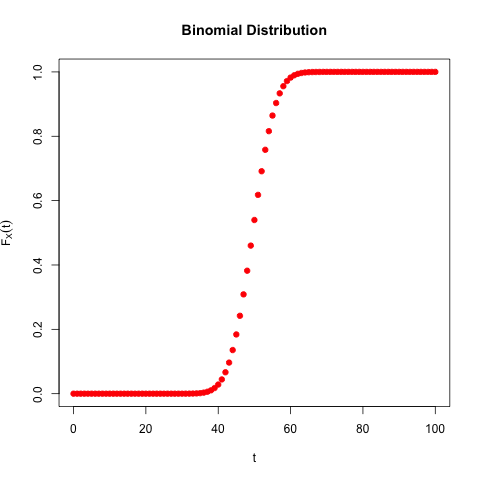
\includegraphics[height=6cm,keepaspectratio]{cdf1.png}

The function $F_X$ is often called the
\emph{cumulative distribution} since it represents the
accumulation of probability as $t$ covers more of the
real axis.  In the figure above for a binomial
cumulative distribution for 100 trials of a fair coin,
we can see that probability of observing less than 40
heads is close to zero.  The probability of observing
less than 60 is close to one.  That tells us that the
most likely scenarios are between 40 and 60.

\subsection{Discrete Densities}

\emph{Discrete distributions} describe experiments where the
random variable takes on discrete values.  These are
often associated with counts.  Their notation will often
be written as $P(X \le n)$ to emphasize the discrete character
of $n$. (Note that $n$ doesn't have to be an integer.)

A \emph{discrete density} $f_X$ corresponding to a discrete
distribution $F_X$ assigns a probability to each discrete value
of the random variable.  If the random variable only takes
integer values, then the density and the distribution
are related in the following ways.

\begin{eqnarray*}
f(n) & = & F(n) - F(n-1)\\
F(n) & = & \sum_{i \le n} f(i)\\
\sum_{i=-\infty}^{\infty} f(i) & = & 1
\end{eqnarray*}

The X subscripts were dropped for brevity; but in general
one writes $F_X$ or $f_X$ to associate the function with
the associated random variable $X$.  This becomes more
important when multiple random variables are considered.

Many useful quantities can be expressed in terms of a density.
First, there is the \emph{mean}.

\begin{equation} \label{discrete_mean}
E[X] = \sum_{i = -\infty}^{\infty} i \cdot f_X(i)
\end{equation}

And the variance.

\begin{equation} \label{discrete_var1}
\mbox{Var}[X] = \sum_{i = -\infty}^{\infty} (i - E(X))^2 \cdot f_X(i)
\end{equation}

A popular alternative expression for the variance can be
obtained by expanding the square.

\begin{eqnarray}
\mbox{Var}[X] & = & \sum_{i=-\infty}^{\infty} (i - E[X])^2 \cdot f_X(i) \nonumber \\
   & = & \sum_{i=-\infty}^{\infty} (i^2 - 2iE[X] + E[X]^2) \cdot f_X(i) \nonumber \\
   & = & \sum_{i=-\infty}^{\infty} i^2 \cdot f_X(i) 
       - 2E[X] \sum_{i=-\infty}^{\infty} i \cdot f_X(i)
       - E[X]^2 \sum_{i=-\infty}^{\infty} f_X(i) \nonumber \\
   & = & E[X^2] - 2E[X] E[X] - E[X]^2 \nonumber \\
   & = & E[X^2] - E[X]^2   \label{discrete_var2}
\end{eqnarray}

This is often expressed in words as ``the mean squared minus the
square of the mean.''  In the special case where the mean is zero,
the variance is equal the mean squared.

The mean is a special cases of a \emph{moments}.
The $n^{\mbox{th}}$ moment is defined as

$$
E[X^n] = \sum_{i = -\infty}^{\infty} i^n \cdot f_X(i)
$$

We've already seen that the first moment is the mean.
The second moment can be used to determine the variance.
Higher moments are not
discussed as often, but they still come in handy.  The
third moment is related to the \emph{skew}, which describes
the degree
to which a distribution is lopsided with respect to its
mean.  The fourth moment is related to the \emph{kurtosis}.  It
describes the extent to which a distribution avoids its mean.

An important tool used in working with distributions is the
\emph{moment generating function}.  For a discrete random
variable, it's defined as

\begin{equation} \label{discrete_mgf}
m_X(t) = E(e^{it}) = \sum_{i=-\infty}^{\infty} e^{it} f_X(i)
\end{equation}

At first glance it looks like way more trouble than it could
possibly be worth.  But moment generating functions turn out
to be important both practically and theoretically.

The theoretical importance derives from analytic function
theory which describes a class of functions that are completely
determined in some neighborhood of a point by the derivatives 
of all orders at the point.  Moment generating functions are
used to show how, in most cases, a distribution is uniquely
determined by the value of all its moments.  This result
is encountered in many proofs to show how a particular
distribution is, in fact, equal to a known distribution.

The practical use is that moment generating functions
often simplify the symbolic calculation of the mean and
variance for many distributions.  The results we need
for the mean and variance are the following.

Given $m_X(t)$ as described in (\ref{discrete_mgf}), the
first and second moments of X are, respectively,

\begin{eqnarray}
E(X) & = & m_X'(0) \label{discrete_mgt_d1} \\
E(X^2) & = & m_X''(0) \label{discrete_mgt_d2}
\end{eqnarray}

It's not immediately obvious how this makes things any
easier.  The examples below will bear it out.

\subsubsection{Binomial Distribution}

We've been using the binomial distribution as an example
for much of the introduction.  Recall that the experiment is that
we perform a sequence of $n$ independent Bernoulli trials, each
of which has probability $p$ of being successful.  The outcome is
the number of successful trials.  Let's consider what the
binomial density looks like.

Let $i$ be the number of successes.  Since $i$ is a count between
zero and $n$, $i$ cannot be less than zero or greater than $n$.  So

$$
p(i) = 0, i \not\in 0, 1, 2, \ldots n
$$

For $i \in 0 \ldots n$ there are $i$ successes and $n-i$ failures.
The probability of such a sequence is $i^p \cdot (n-i)^{(1-p)}$
since each outcome is independent of the one before it.  We then
have to account for the number of positions the $i$ occurrences
could have occurred among the $n$ trials.  There are $n$ ways to
pick the first one.  For each one of these, there are $n-1$ ways
to pick the next one.  This continues until we have picked $i$
times down to $n-i+1$.  This leads to the following expression
with $i$ factors for the $i$ chosen positions.

$$
n \cdot n-1 \cdots n-i+1
$$

But this product distinguishes between the order of the successes.
For example, if the first two are successes, it counts first then
second separately from second and then first.  The order doesn't
matter.  So we divide by the number of permutations of $i$ elements,
which is $i!$: $i$ ways to choose the first one, $i-1$ ways to
choose the second one, down to 1.  So the number of ways we
can choose $i$ elements from $n$ elements without replacement
divided by the number of ways we could have ordered $i$ elements,
we get 

\begin{eqnarray*}
\frac{n(n-1) \cdots (n-i+1)}{i!} & = & \frac{n(n-1) \cdots (n-i+1)}{i!} \cdot
         \frac{n-i}{n-i} \cdot \frac{n-i-1}{n-i-1} \cdots 
         \frac{2}{2} \cdot \frac{1}{1} \\
      & = & \frac{n!}{i! (n-i)!} \\
      & = & {n \choose i}
\end{eqnarray*}

The notation in the last expression is read ``$n$ choose $i$''.

Whew!

So a particular occurrence of $i$ successes and $n-i$
failures occurs with probability $p^i \cdot (1-p)^{n-i}$.
Since there are ${n \choose i}$ ways this can happen, the
probability this can happen in \emph{some way} 
(whichever order, we don't care) is

\begin{equation} \label{binomial_density}
f(i) = {n \choose i} p^i (1-p)^{n-i}, i \in 0, \ldots, n
\end{equation}

This is a probability, the sum of all possible values
should add to one.  Using the binomial formula, we have

\begin{eqnarray*}
\sum_{i=-\infty}^{\infty} f(i) & = & \sum_{i=0}^{n} f(i) \\
   & = & \sum_{i=0}^{n} {n \choose i} p^i (1-p)^{n-i}  \\
   & = & [ p + (1-p) ]^2 \\
   & = & 1^2
\end{eqnarray*}

Great! The probabilities sum to one.  Now let's evaluate
the mean and variance of this distribution.  From
(\ref{discrete_mean}) we have to evaluate

$$
\sum_{i=0}^n i {n \choose i} p^i (1-p)^{n-i}
$$

This is not easy to solve in a closed form.  It's
one of those times where we appeal to the moment generating
function.

\begin{eqnarray*}
m_X(t) & = & E(e^{it}) \\
   & = & \sum_{i=0}^n e^{it} {n \choose i} p^i (1-p)^{(n-i)} \\
   & = & \sum_{i=0}^n {n \choose i} (pe^t)^i (1-p)^{(n-i)} \\
   & = & (pe^t + 1 - p)^n \\
   & = & (pe^t + q)^n
\end{eqnarray*}

In the last step, $1-p$ is replaced with $q$.  We just
remember that $p + q = 1$.  Now
differentiate the moment generating function twice with
respect to $t$.

\begin{eqnarray*}
m_X'(t) & = & n(pe^t + q)^{(n-1)} pe^t \\
m_X''(t) & = & n(n-1)(pe^t + q)^{(n-2)} pe^t pe^t +
          n(pe^t + q)^{(n-1)} pe^t \\
   & = & npe^t(pe^t + q)^{(n-2)}((n-1)pe^t + pe^t + q) \\
   & = & npe^t(pe^t + q)^{(n-2)}(npe^t + q)
\end{eqnarray*}

And evaluate each of the derivatives at $t=0$ for the
required moments.

\begin{eqnarray*}
E(X) & = & m_X'(0) \\
   & = & n(pe^0 + q)^{n-1} pe^0 \\
   & = & n(p+q)^{n-1}p \\
   & = & n1^{n-1}p \\
   & = & np  \\
E(X^2) & = & m_X''(0) \\
   & = & npe^0(pe^0 + q)^{(n-2)}(npe^0 + q) \\
   & = & np(p+q)^{n-2} (np + q) \\
   & = & np (np+q) \\
   & = & (np)^2 + npq
\end{eqnarray*}

The mean is $np$ like we would expect.  For the variance,
substitute these values into (\ref{discrete_var2}).

\begin{eqnarray}
\mbox{Var}(X) & = & E(X^2) - E(X)^2 \nonumber \\
   & = & (np)^2 + npq - (np)^2 \nonumber \\
   & = & npq \label{binomial_var}
\end{eqnarray}

\subsubsection{Poisson Process}
\label{subsec:poisson}

A Poisson process is a special type of counting process.
A counting process is a function $N(t), t \ge 0$ that
only takes non-negative integer values, is non-decreasing,
and $N(0)=0$;
i.e. it represents a count of occurrences over time.  The
Python and R workshops provide graphs of the Poisson
probability mass function.

\begin{equation} \label{poisson_pmf}
f_X(k; \lambda) = e^{-\lambda} \frac{\lambda^k}{k!} 
\quad k = 0, 1, 2, \ldots
\end{equation}

The workshops experiment with $\lambda = 5$.  You get a
PMF curve with a hump near $\lambda$.

\textbf{Mean and Variance}

For the mean and variance we appeal once again to the
moment generation function technique.

\begin{eqnarray*}
m_X(t) & = & E(e^{it}) \\
   & = & \sum_{i=0}^n e^{it} e^{-\lambda} \frac{\lambda^k}{k!} \\
   & = & e^{-\lambda} \sum_{i=0}^n \frac{(e^t \lambda)^i}{i!} \\
   & = & e^{-\lambda} e^{e^t \lambda}
\end{eqnarray*}

Now differentiate the moment generating function twice with
respect to $t$.

\begin{eqnarray*}
m_X'(t) & = & e^{-\lambda} e^{e^t \lambda} e^t \lambda \\
        & = & \lambda e^{(t-\lambda) + \lambda e^t} \\
m_X''(t) & = & \lambda e^{(t-\lambda) + \lambda e^t}(1+\lambda e^t)\end{eqnarray*}

Now evaluate each of the derivatives at $t=0$ for the
required moments.

\begin{eqnarray*}
E(X) & = & m_X'(0) \\
   & = & \lambda e^{(0-\lambda) + \lambda e^0} \\
   & = & \lambda e^0 \\
   & = & \lambda \label{poisson_mean} \\
E(X^2) & = & m_X''(0) \\
   & = & \lambda e^{(0-\lambda) + \lambda e^0}(1+\lambda e^0) \\
   & = & \lambda e^0(1+\lambda) \\
   & = & \lambda + \lambda^2
\end{eqnarray*}

The mean is $\lambda$ like we expect.  For the variance we
substitute these values into (\ref{discrete_var2}).

\begin{eqnarray}
\mbox{Var}(X) & = & E(X^2) - E(X)^2 \nonumber \\
   & = & \lambda + \lambda^2 - \lambda^2 \nonumber \\
   & = & \lambda \label{poisson_var}
\end{eqnarray}

\textbf{Motivation}

The curve looks plausible
enough.  But why this function?  Is it just the most
convenient way to express a curve with a hump in a certain
place?  Or is there something special about the expression
in (\ref{poisson_pmf})?

It turns out that this particular "humped curve" does indeed
have some special properties.  In fact, (\ref{poisson_pmf})
can be derived from four properties.

\begin{enumerate}  \label{poisson_properties}

\item Non-overlapping intervals are independent.

\item The processes is \emph{stationary}.  That is,
  the probability of an occurrence within time $h$
  from zero is the same as the probability of an occurrence
  within time $t$ to $t + h$, it doesn't depend on $t$.
  In symbols: $P[N(t+h)-N(t)]$ depends only on $h$, not $t$.
  
\item $P[N(t) = 1] = \lambda t + o(t)$

\item $P[N(t) > 1] = o(t)$

\end{enumerate}

The symbol $o(t)$ represents any quantity second order or
higher.  Namely,

$$
\lim_{t \rightarrow 0} \frac{o(t)}{t} = 0
$$

If $o(t)$ was analytic (and we're not saying it is), then
its power series representation would only have second
order and above terms (i.e. $o(t) = a_2t^2 + a_3t^3 \ldots$).

  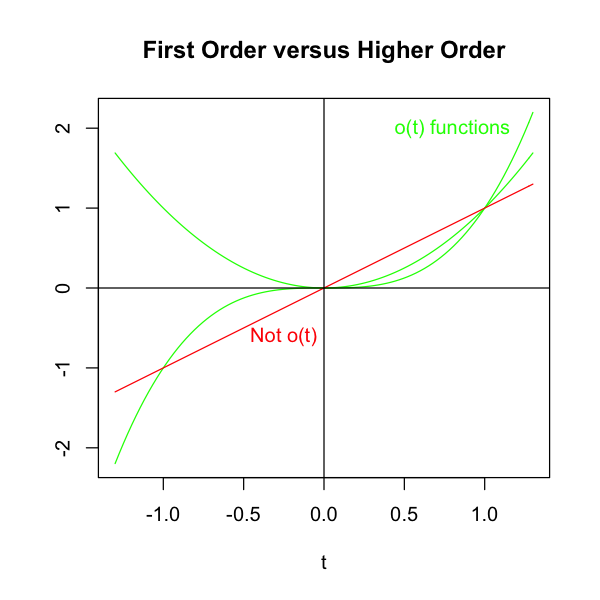
\includegraphics[height=8cm,keepaspectratio]{ot.png}

Conditions 3 and 4 are saying that $P[N(t) = 1]$ is similar
to the red line for small $t$ while $P[N(t) > 1]$
looks like a linear combination of green lines.

\subsection{Continuous Distributions}

\emph{Continuous distributions} describe experiments where
the random variable can take continuous values.  Examples
are time intervals and averages of counts.

A \emph{continuous density} $f_X$ corresponding to a continuous
distribution is related through its integral in a way similar to
how a discrete mass function is related through a sum.

\begin{eqnarray*}
F_X(x) & = & \int_{-\infty}^x f(t) dt \\
f_X(x) & = & \frac{dF(x)}{dx}
\end{eqnarray*}

The analogous formulas for expectation and variance also hold.

\begin{eqnarray}
E[X] & = & \int_{-\infty}^{\infty} xf_X(x) dx \label{cont_mean} \\
\mbox{Var}[X] & = & \int_{-\infty}^{\infty} (E[X] - x)^2 f_X(x) dx \label{cont_var}
\end{eqnarray}

Our friend, the moment generating function, continues to be useful
with continuous random variables.

\begin{equation} \label{cont_mgf}
m_X(t) = E[e^{xt}] = \int_{-\infty}^{\infty} e^{xt} f_X(x) dx
\end{equation}

This is the continuous version of (\ref{discrete_mgf}).

\subsubsection{Normal Distribution}

The granddaddy of all distributions is the \emph{normal distribution}.
It has two parameters: the mean $\mu$ and standard deviation
$\sigma$.  The density function for the normal distribution in one
dimension is given by the following formula.

\begin{equation}
f_X(x; \mu, \sigma) = \frac{1}{\sqrt{2\pi}\sigma}e^{\frac{-(x - \mu)^2}{2\sigma^2}}
\end{equation}

It has the familiar bell-shaped curve centered about the mean.
A common practice is to normalize the random variable through
the transformation

$$
z = \frac{x - \mu}{\sigma}
$$

Then it takes the form

\begin{equation}
f_X(z) = \frac{1}{\sqrt{2\pi}}e^\frac{-z^2}{2}
\end{equation}

The moment generation function is defined in the usual way.

\begin{eqnarray*}
m_X(t) &= &E \left[ e^{tx}\right] \\
  &= &\int_{-\infty}^{\infty} e^{tx} \frac{1}{\sqrt{2\pi}\sigma} 
         e^{-\frac{(x-\mu)^2}{2\sigma^2}} dx \\
  &= &\frac{1}{\sqrt{2\pi} \sigma} \int_{-\infty}^{\infty}
       \exp \left[ -\frac{1}{2} \left( \frac{x-\mu}{\sigma} \right)^2 + tx \right] dx
\end{eqnarray*}

From this point it becomes an exercise in completing the square within
the exponent.

\begin{eqnarray*}
-\frac{1}{2} \frac{(x-\mu)^2}{\sigma^2} + tx & = & \frac{1}{2\sigma^2} \left[
      (x-\mu)^2 - 2tx\sigma^2 \right] \\
   &= &\frac{1}{2\sigma^2} \left[ x^2 - 2x\mu + \mu^2 - 2tx\sigma^2 \right] \\
   &= &\frac{1}{2\sigma^2} \left[ x^2 - 2x(\mu + t\sigma^2) + \mu^2 \right] \\
   &= &\frac{1}{2\sigma^2} \left[ [ x^2 - 2x(\mu + t\sigma^2) + (\mu + t\sigma^2)^2 ]
       - (\mu + t\sigma^2)^2 + \mu^2 \right] \\
   &= &\frac{1}{2\sigma^2} \left[ [x - (\mu + t\sigma^2)]^2
       - \mu^2 + 2\mu t \sigma^2 - t^2 \sigma^4 + \mu^2 \right] \\
   &= &\frac{1}{2} \left[ \frac{x - (\mu + t\sigma^2)}{\sigma} \right]^2
      +\frac{1}{2} \left[ 2\mu t + t^2 \sigma^2 \right]
\end{eqnarray*}

Now if we substitute this exponent expression back into our moment
generating function, we get

\begin{eqnarray}
m_X(t) &= &\frac{1}{\sqrt{2\pi} \sigma} \int_{-\infty}^{\infty} \exp \left[
   \frac{1}{2} \left( \frac{x - (\mu + t\sigma^2)}{\sigma} \right)^2
      +\frac{1}{2} ( 2\mu t + t^2 \sigma^2) \right] dx  \nonumber \\
  &= &\exp \left[ \frac{1}{2} ( 2\mu t + t^2 \sigma^2) \right] \frac{1}{\sqrt{2\pi} \sigma} 
   \int_{-\infty}^{\infty} \exp \left[ \frac{1}{2} 
   \left( \frac{x - (\mu + t\sigma^2)}{\sigma} \right)^2 \right] dx \nonumber \\
  &= & \exp \left[\mu t + \frac{1}{2}t^2 \sigma^2 \right] \label{norm_mgf}
\end{eqnarray}

Now differentiate $m_X(t)$ twice.

\begin{eqnarray*}
m_X'(t) &= &(\mu + t\sigma^2) \exp \left[ \mu t + \frac{1}{2} t^2 \sigma^2 \right] \\
m_X''(t) &= &(\mu + t\sigma^2) (\mu + t\sigma^2) 
   \exp \left[ \mu t + \frac{1}{2} t^2 \sigma^2 \right]
   + \sigma^2 \exp \left[ \mu t + \frac{1}{2} t^2 \sigma^2 \right]
\end{eqnarray*}

Evaluate at zero to obtain the moments.

\begin{eqnarray*}
E[X] &= &m_X'(0) \\
   &= &(\mu + 0) \exp [0] \\
   &= &\mu \\
E[X^2] &= &m_X''(0) \\
   &= &(\mu + 0) (\mu + 0) \exp[ 0] + \sigma^2 \exp [0] \\
   &= &\mu^2 + \sigma^2
\end{eqnarray*}

The variance comes out as expected.

\begin{eqnarray*}
\mbox{var}[X] &= &E[X^2] - E[X]^2 \\
  &= &\mu^2 + \sigma^2 - \mu^2 \\
  &= &\sigma^2
\end{eqnarray*}


A linear combination of normal distributions
$X_1, X_2, ..., X_n$ are \emph{jointly normal}
if the density of linear combination is given by

$$
\frac{1}{(\sqrt{2\pi})^n} \frac{1}{\mbox{det}|G|} \exp
\left[ -\frac{1}{2}(x-\alpha)^t G^{-1} (x-\alpha) \right]
$$

This seems menacing at first.  But we can gain an
intuition for it if we consider some simple cases.
Perhaps the most menacing introduction is the
correlation matrix $G$.  This matrix contains the covariance
of each pair of $X_i$.

$$
G_{ij} = \mbox{cov}(X_i, X_j)
$$

Let's consider the case where the $X_i$ are independent of
each other.  Then $\mbox{cov}(X_i, X_j) = 0$ for $i \ne j$
and G is diagonal where each diagonal element
$G_{ii} = var(X_i) = \sigma_i^2$.

Let's assume the $X_i$ are centered so that $\alpha = 0$.
Then the expression in the exponent simplifies to

\begin{eqnarray*}
-\frac{1}{2}(x-\alpha)^t G^{-1} (x-\alpha) &= &-\frac{1}{2} x^t G^{-1} x \\
  &= &-\frac{1}{2} \sum_{i=1}^n x_i \frac{1}{G_{ii}} x_i \\
  &= &-\frac{1}{2} \sum_{i=1}^n \frac{x_i^2}{G_{ii}}
\end{eqnarray*}

With these simplifications, the exponent becomes a weighted
some of squares among the $x$ components.  If we further
stipulate that the variances are equal, then $G = \sigma^2 I$
is a constant and the expression simplifies to

$$
-\frac{1}{2} \sum_{i=1}^n \frac{x_i^2}{\sigma^2} =
-\frac{1}{2\sigma^2} \sum_{i=1}^n x_i^2 =
-\frac{1}{2} \frac{|x|^2}{\sigma^2}
$$

So we can see how the general form simplifies to our
familiar one if we make assumptions about covariances.

\subsubsection{Exponential Distribution}

The Exponential distribution is, in a sense, the complement of
the Poisson distribution introduced in 
Subsection (\ref{subsec:poisson}).  Whereas the Poisson
distribution applies to the question of ``how many occurrences
of an event happen per unit time for Poisson process,'' 
the Exponential distribution addresses the question 
``how long until the next occurrence.''

Let's get a feel for how the characterization of a Poisson 
process from
Page (\pageref{poisson_properties}) leads to an Exponential
distribution.  Let $P_0(t)$ denote the probability of no
occurrences between times 0 and $t$.  We can rewrite this
in terms of characterics (iii) and (iv) of a Poisson process.

\begin{eqnarray*}
P_0(t) &= & \mbox{nothing happens from zero to time} \: t \\
  &= & 1 - [\mbox{exactly one thing happens}] - 
     [ \mbox{more than one thing happens} ] \\
  &= & 1 - [\lambda t) + o(t)] - [ o(t) ] \\
  &= & 1 - \lambda t + o(t)
\end{eqnarray*}

The $o(t)$ arithmetic may look funny.  But remember that $o(t)$
refers to a class of functions which are closed under linear
combinations.

Another property that $P_0(t)$ has from Poisson characteristic
(i) of Page \pageref{poisson_properties} is that non-overlapping
intervals are independent.  That means the probability of two
things happening in separate (non-overlapping) intervals is the
product of the separate probabilities.

$$
P_0(t+h) = P_0(t)P_0(h)
$$

We can the above two equations to derive a differential equation
for $P_0(t)$.

\begin{eqnarray}
\frac{dP_0(t)}{dt} &= & \lim_{h \to 0} \frac{P_0(t+h) - P_(t)}{h} \nonumber \\
  &= & \lim_{h \to 0} \frac{P_0(t)P_0(h) - P_0(t)}{h} \nonumber \\
  &= & \lim_{h \to 0} \frac{P_0(t)(P_0(h) - 1)}{h} \nonumber \\
  &= & P_0(t)\lim_{h \to 0} \frac{(1 - \lambda h + o(h) - 1)}{h} \nonumber \\
  &= & P_0(t)\left[ \lim_{h \to 0} \frac{-\lambda h}{h} 
     + \lim_{h \to 0} \frac{o(h)}{h} \right] \nonumber \\
  &= & P_0(t)\left[ \lim_{h \to 0} (-\lambda)
     + 0 \right] \nonumber \\
  &= & -\lambda P_0(t) \label{exp_de}
\end{eqnarray}

This first order differential equation has a well known solution
of $P_0(t) = Ke^{\lambda t}$ for arbitrary constant $K$.  Since
we are constraining $P_0(t)$ to be a probability density function,
we require that

$$
1 = \int_0^{\infty} K e^{-\lambda t}
$$

which constrains $K$ to be $\lambda$.  This applies at a
particular point $t$.  But since the Poisson process is
\emph{stationary} 
(characteristic (ii) on Page \pageref{poisson_properties})
it translates to all $t > 0$.  So our expression for the
exponential density of a Poisson process with rate $1/\lambda$
is

\begin{equation} \label{exp_density}
f_X(x; \lambda) = \lambda e^{-\lambda x}
\end{equation}

The exponential random variable has a cumulative distribution
function of the form

\begin{equation} \label{exp_cdf}
F_X(x; \lambda) = \left\{ \begin{array}{r@{\quad:\quad}l}
   1 - e^{-\lambda x} & x > 0 \\
   0 & x \le 0
 \end{array} \right.
\end{equation}


To calculate the mean and variance, we resort once again to the
moment generating function.

\begin{eqnarray}
m_X(t) & = & E[e^{xt}] \nonumber \\
   & = & \int_0^{\infty} e^{xt} \lambda e^{-x \lambda} dx \nonumber \\
   & = & \lambda \int_0^{\infty} e^{-x(\lambda - t)} dx \nonumber \\
   & = & \left. \lambda \cdot \frac{-1}{\lambda - t} e^{-x(\lambda - t)}
      \right|_{x=0}^{x=\infty} \nonumber \\
   & = & \frac{-\lambda}{\lambda - t} (0 - 1) \nonumber \\
   & = & \frac{\lambda}{\lambda - t} \label{exp_mgf}
\end{eqnarray}

Note the definite integral only converges for $\lambda - t > 0$.
This is fine for our needs since we intend to evaluate the moment
generating function close to zero for its derivatives at zero.

Now differentiate the moment generating function twice with
respect to $t$.

\begin{eqnarray*}
m_X'(t) & = & \lambda(\lambda - t)^{-2}  \\
m_X''(t) & = & \lambda (-2)(\lambda - t)^{-3}(-1) \\
   & = & \frac{2 \lambda}{(\lambda - t)^3}
\end{eqnarray*}

Now evaluate each of the derivatives at $t=0$ for the
required moments.

\begin{eqnarray}
E(X) & = & m_X'(0)
   = \frac{\lambda}{\lambda^2}
   = \frac{1}{\lambda} \label{expon_mean} \\
E(X^2) & = & m_X''(0) 
   = \frac{2 \lambda}{\lambda^3}
   = \frac{2}{\lambda^2} \nonumber
\end{eqnarray}

The mean is $1 / \lambda$.  For the variance we
substitute these values into (\ref{discrete_var2}).

$$
\mbox{Var}(X) = E(X^2) - E(X)^2
   = \frac{2}{\lambda^2} - \frac{1}{\lambda^2}
   = \frac{1}{\lambda^2} \label{expon_var}
$$

It turns out the first and second moments are not difficult
to derive directly from their integral formulas.

\begin{eqnarray*}
E[X] & = & \int_0^{\infty} x \lambda e^{-\lambda x} dx \\
E[X^2] & = & \int_0^{\infty} x^2 \lambda e^{-\lambda x} dx
\end{eqnarray*}

It's a straight forward pair of calculations using integration
by parts. But moment generating functions still save a little
bit of work.

\subsubsection{Gamma Distribution}

The \emph{Gamma function} is defined by

\begin{equation} \label{gamma_function}
\Gamma(r) = \int_{0}^{\infty} x^{r-1} e^{-x} dx
\end{equation}

for $r \in [1,\infty)$.
One application of integration by parts reveals its
special property.

\begin{eqnarray*}
\Gamma(r) &= &\int_{0}^{\infty} x^{r-1} e^{-x} dx \\
  &= &\left. -x^{r-1}e^{-x} \right|_0^{\infty}
     + \int_0^{\infty} (r-1)x^{r-2} e^{-x} dx \\
  &= &-(0 - 0) + (r-1) \int_0^{\infty} x^{(r-1) - 1} e^{-x} dx \\
  &= &(r-1) \Gamma(r-1) \\
\end{eqnarray*}

It's easy to show $\Gamma(1)=1$.  So for positive integers
$\Gamma(n) = (n-1)\Gamma(n-1) = (n-1)!$.  But the Gamma function
is defined for all real $r>1$.  So the special property of the
Gamma function is that it
``fills in the gaps'' of the factorial function.

The Gamma function lends its name to the
\emph{Gamma density function}.

\begin{equation} \label{gamma_density}
\mbox{Gamma}(x; r, \lambda) = \frac{\lambda}{\Gamma(r)} 
     (\lambda x)^{r-1} e^{- \lambda x}
\end{equation}

We'll see in the next section how the Gamma random variable
arises from summing $r$ Exponential random variables with
parameter $\lambda$.
For now let's content ourselves with determining its moment
generating function.  About halfway through you see the change
of variable $u = (\lambda - t)x$.

\begin{eqnarray}
m_X(t) & = & E[e^{xt}] \\
   & = & \int_0^{\infty} e^{xt} \frac{\lambda}{\Gamma(r)} 
     (\lambda x)^{r-1} e^{- \lambda x} dx \nonumber \\
   &= & \frac{\lambda}{\Gamma(r)} \int_0^{\infty} (\lambda x)^{r-1}
    e^{-(\lambda - t)x} dx \nonumber \\
   & = & \frac{\lambda}{\Gamma(r)} \int_0^{\infty} 
        \left( \frac{\lambda u}{\lambda - t} \right)^{r-1}
        e^{-u} \frac{du}{\lambda - t} \nonumber \\
   & = & \frac{\lambda^r}{(\lambda - t)^r \Gamma(r)} \int_0^{\infty} 
        u^{r-1}  e^{-u} du \nonumber  \\
   & = & \frac{\lambda^r \Gamma(r)}{(\lambda - t)^r \Gamma(r)} \nonumber \\
   & = & \left( \frac{\lambda}{\lambda - t} \right)^r \label{gamma_mgf}
\end{eqnarray}

This reduces to ($\ref{exp_mgf}$) for the Exponential distribution
when $r=1$.


\section{Random Variable Functions}

Most of the random variables we've examined so far directly
directly model some conceptually simple experiment like
flipping a coin, counting the successes of a number of trials,
or counting the number of occurrences over a fixed time interval.
But we'll find there is value in constructing new random variables
that are functions of random variables we have already encountered.
The most common cases are squares and linear
combinations of variables.  This section will outline two
techniques useful for determining the distribution function
that arises from a function of a random variable.

\subsection{CDF Method}

Consider random variable $Y = X^2$ where we already know
the density function $f_X(x)$. What can we say about $f_Y(y)$.
The technique we'll demonstrate in this section starts with
the CDF.  Since $Y$ can only take on positive values, we know
that the CDF is zero for all $Y \le 0$.

Let's recall what a random variable is doing.
A random variable maps from an abstract event space to points on
the real number line.  Often the event space won't be so abstract
and the mapping will be quite natural; so natural that we often just
write $X$ rather than
$X(\omega) \in \mathcal{R}$ for $\omega \in \Omega$.

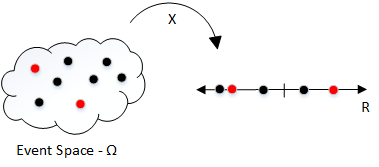
\includegraphics[width=\linewidth]{rv1.png}

By mapping from an ``event space'' to the concrete real number line,
random variables allow us to directly employ analytic techniques
that have long existed for the real number line.  Our
cumulative distribution functions and probability density functions
are defined on the real number line by virtue of the random variable
that maps events to the real number line.

A function of a random variable simply maps the points from one
real number line to another real number line.  In this way, a function
of a random variable creates a new random variable on the same event
space, i.e. a new way to map events to real numbers.

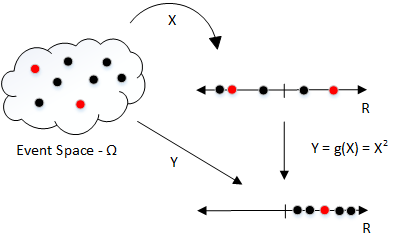
\includegraphics[width=\linewidth]{rv2.png}

In the figure above, $g(x) = x^2$ is such a function.  If we define
$Y$ as the result of mapping
$\Omega \rightarrow \mathcal{R} \rightarrow \mathcal{R}$, then
$Y$ is also a random variable.

Assuming that such a mapping is useful (and we'll find out later that
this $g(X) = X^2$ is), we'll want to know the CDF and PDF of the new
random variable.  Unfortunately, it's not as simple as plugging
$x^2$ everywhere you see an $x$.

Using the figure above as an example, let's determine $F_Y(y)$ from
basic principles.  The basic principle is

$$
F_Y(y) = P[Y \le y]
$$

From this principle we plug in the function to derive the expression.
Since $Y = g(X) = X^2$, we restrict our attention to $y > 0$ since
$F_Y(y) = 0$ for $y \le 0$.

\begin{eqnarray*}
F_Y(y) &= &P[Y \le y] \\
  &= &P[X^2 \le y] \\
  &= &P\left[-\sqrt{y} \le X \le \sqrt{y}\right] \\
  &= &P\left[X \le \sqrt{y}\right] - P\left[X \le -\sqrt{y}\right]
\end{eqnarray*}

This gives us the CDF for Y.  It's close to simply substituting
$\sqrt{y}$ for $x$ into the expression for $F_X$.  Now that we have
the CDF, we can derive the PDF.

\begin{eqnarray*}
f_Y(y) &= &\frac{d}{dy}F_Y(y) \\
   &= &\frac{d}{dy}\left[ F_x(\sqrt{y}) - F_X(-\sqrt{y}) \right] \\
   &= &\left. \frac{dF_X}{dx} \right\vert_{x=\sqrt{y}} \frac{d(\sqrt{y})}{dy} - 
   \left. \frac{dF_X}{dx} \right \vert_{x=-\sqrt{y}} \frac{d(-\sqrt{y})}{dy} \\
   &= &\frac{1}{2\sqrt{y}} \left[ f_x(\sqrt{y}) + f_x(-\sqrt{y}) \right]
\end{eqnarray*}

where

$$
\frac{dx}{dy} = \frac{d y^{\frac{1}{2}}}{dy} = \frac{1}{2}y^{-\frac{1}{2}}
$$

The expression for $f_Y$ in terms of $f_X$ in this specific case of
$Y = X^2$ demonstrates two important complications.

1. If $g$ is not 1-to-1, then we must account for all the points
   in $g^{-1}(y)$.  In the case of a quadratic, there are usually
   two.

2. The $f_Y$ expression introduced an additional multiplicative
   factor, known in vector calculus circles as \emph{the Jacobian}.
   The Jacobian incorporates the stretch factor introduced by the
   transformation.

It's reasonable to ask why the CDF didn't need a stretch factor.
It's because we don't integrate the CDF.  We just evaluate it at
various points.
\textbf{The value of the CDF at any point represents a probability.}

This is not the case with a continuous density function.  The
value of $f_X$ at a single point does not really mean anything
\textbf{by itself.
It certainly does not represent a probability.}  We only get
probabilities from $f_X$ by integrating it over some interval
or combination of intervals.  In other words, it's only the
area under $f_X$ that has a probability interpretation.  You
can't say anything about an area with just the height.  You
need to also specify the width.  So in the case of our transformation
$g$, it's not enough to determine the height of $f_Y$ at a certain
point through corresponding values of $f_X$.  We need to know how
$g$ is stretching the differential widths to get the full picture
of how areas under $f_X$ transform to \emph{areas} under $f_Y$.  The
Jacobian factor provides this ``width stretching'' information.

We're still messing around in the realm of probability.  In the next
workshop, we'll consider some special functions of a random
variable (like the average of a sample) and cross into the
realm of \emph{statistics} proper.

\subsection{Moment Generating Functions}

Another way to determine the density function $f_Y(y)$ for
$Y = g(X)$ is to compute the moment generating function of
$g(x)$ and determine whether it's something we recognize.

\subsubsection{Linear Combinations}

Let's consider the case where we have $n$ independent samples,
each one from its own distribution.  Let $Y$ be a linear
combination of the independent samples.  That is,
$Y = g(X) = a_1 X_1 + \cdots + a_n X_n$ where $X_i$
represents the distribution $i$ from which we are sampling.
The $a_i$ are constants.
The expression for the moment generating function is

\begin{eqnarray}
m_Y(t) &= & E \left[ e^{tY} \right] 
  =  E \left[ e^{tg(x)} \right] 
  = E \left[ e^{t \sum_{i=1}^n a_i X_i} \right]
  = E \left[ e^{\sum_{i=1}^n t a_i X_i} \right]
  = E \left[ \prod_{i=1}^n e^{t a_i X_i} \right] \nonumber \\
  &= & \prod_{i=1}^n E \left[ e^{t a_i X_i} \right]
  = \prod_{i=1}^n m_{X_i}(t a_i) \label{mgf_product}
\end{eqnarray}

We used the independence between the samples in going from the
first line to the second.
So the moment generating function for the sum of independent 
random variables can be expressed as product of the individual
moment generating function.

Let's consider an example where $X$ represents an exponential
random variable with parameter $\lambda$.  Recall that the
value of the exponential random variable is the expected wait
time for a Poisson process with rate $1/\lambda$.  Let
$Y = X_1 + \cdots + X_n$, the time for the $n$th occurrence.
Then the product rule in ($\ref{mgf_product}$) where each
$m_{X_i}$ is the exponential moment generating function with
parameter $\lambda$.  We established this in
Equation ($\ref{exp_mgf}$) on Page $\pageref{exp_mgf}$.

$$
m_X(t) = \frac{\lambda}{\lambda - t}
$$

Plugging this into ($\ref{mgf_product}$) yields

$$
m_Y(t) = \prod_{i=1}^n m_{X_i}(t)
  = \prod_{i=1}^n \frac{\lambda}{\lambda - t}
  = \left( \frac{\lambda}{\lambda - t} \right)^n
$$

And this, as we saw in Equation ($\ref{gamma_mgf}$) on
Page $\pageref{gamma_mgf}$, is the moment generating
function for the Gamma distribution.

Another popular application of ($\ref{mgf_product}$)
yields the moment generating function for an average of
independent samples.

$$
\bar{X} = \frac{1}{n} \sum_{i=1}^n X_i
$$

In this case, we have $X_i = X$ and $a_i = 1/n$.

\begin{equation}
m_{\bar{X}}(t) = \left[ m_X \left( \frac{t}{n} \right) \right]^n
\end{equation}

\subsubsection{Normal Squares}

The above are nice general results.  Let's focus our attention
on the normal distribution.  The formulas above apply to
the normal distribution; but here we'll investigate random
variables that arise from the squares of a normal random
variable.

Why would we care about the square of a normal random
variable?  This is actually two questions.

\begin{enumerate}
\item Why do we care about squares?
\item Why do we care about the normal distribution?
\end{enumerate}

We care about the square of the distance from the mean
because it provides us information about the
spread around its mean.  Combinations of
positions arounds its mean can cancel out.
But squares are always positive and they accumulate.
Moreover, they accumulate in expected
patterns which, if not followed, lead us to suspect the
underlying assumptions.
One popular application of this is the so-called Chi-Squared
goodness of fit test.

Consider the case of $n$ independent samples from a normal
distribution with mean $\mu$ and variance $\sigma^2$; then
standardize the usual way.

$$
Z_i = \frac{X_i - \mu}{\sigma}
$$

Our new random variable will be

$$
U = \sum_{i=1}^n Z_i^2 = \sum_{i=1}^n \left( 
    \frac{X_i - \mu}{\sigma} \right)^2
$$

A single value of U represents the outcome of the experiment
of independently sampling the $X$ random variable $n$ times,
squaring each value, and summing these squares.  If we do
this many times, the values of U are distributed in a certain
way.  We don't yet know how to expect these values to be
distributed.  A density function for U would certainly help.
To this end, let's see if we can determine the moment
generating function for U.

\begin{equation}
m_U(t) = E \left[ e^{tU} \right]
 = E \left[ e^{t \sum_{i=1}^n Z_i^2} \right]
 = E \left[ \prod_{i=1}^n e^{t Z_i^2} \right]
 = \prod_{i=1}^n E \left[ e^{t Z_i^2} \right] \label{norm_sq1}
\end{equation}

This is just the linear combination stuff we did in the
last section.  Now let's dig into this square.

\begin{eqnarray}
E \left[ e^{t Z_i^2} \right] &= & \frac{1}{\sqrt{2\pi}}
     \int_{-\infty}^{\infty} e^{tz_i^2} e^{-\frac{1}{2} z_i^2}
     dz_i \nonumber \\
  &= & \frac{1}{\sqrt{2\pi}}
     \int_{-\infty}^{\infty} e^{-\frac{1}{2} (1-2t)z_i^2}
      dz_i \label{norm_sq2}
\end{eqnarray}

At this point we introduce a standard change of variable for
this kind of thing.

\begin{eqnarray*}
u^2 = (1-2t)z_i^2 & \; &2udu = (1-2t)2z_idz_i \\
\frac{u}{z} = \sqrt{1-2t} & \; &dz_i = \frac{2udu}{(1-2t)2z}
    = \frac{\sqrt{1-2t}}{1-2t} du = \frac{du}{\sqrt{1-2t}}
\end{eqnarray*}

Let's dump all this into ($\ref{norm_sq2}$) to get something
we can work with.

\begin{eqnarray}
E \left[ e^{t Z_i^2} \right] &= & \frac{1}{\sqrt{2\pi}}
     \int_{-\infty}^{\infty} e^{-\frac{1}{2} u^2}
      \frac{du}{\sqrt{1-2t}} \nonumber \\
  &= & \frac{1}{\sqrt{1-2t}} \frac{1}{\sqrt{2\pi}}
     \int_{-\infty}^{\infty} e^{-\frac{1}{2} u^2} du \nonumber \\
  &= & \frac{1}{\sqrt{1-2t}}  \nonumber  \\
  &= & \left( \frac{1/2}{1/2 - t} \right)^{1/2} \label{norm_sq3}
\end{eqnarray}

Substitute ($\ref{norm_sq3}$) back into ($\ref{norm_sq1}$).

\begin{eqnarray}
m_U(t) &= &\prod_{i=1}^n \left( \frac{1/2}{1/2 - t} \right)^{1/2}
   \nonumber \\
   &= & \left( \frac{1/2}{1/2 - t} \right)^{n/2}
\end{eqnarray}

Now let's step back and think: have we seen a moment generating
function like this anywhere?  It should look familiar.
If not, review the previous section where we showed how the
Gamma random variable arises from successive exponential trials.
The Gamma moment generating function is 
Equation ($\ref{gamma_mgf}$) on Page $\pageref{gamma_mgf}$.
The expression in ($\ref{norm_sq3}$) is Gamma moment generating
function for $r = n/2$ and $\lambda = 1/2$.

So our sum of squares of standard normals has a distribution
that we have already encountered before: $\mbox{Gamma}(n/2, 1/2)$.
This distribution is special enough to get its own name:
the \emph{Chi Squared} distribution.

\begin{eqnarray} \label{chisq_density}
\chi_n^2(x) = \mbox{Gamma}(x; n/2, 1/2) = \frac{1/2}{\Gamma(n/2)} 
     \left( \frac{x}{2} \right)^{\frac{n}{2}-1} e^{- x/2}
\end{eqnarray}

The $n$ is a parameter of our distribution called the
\emph{degrees of freedom}.  So the above expression is
spoken as a 
"Chi-Squared distribution with n degrees of freedom."

\subsection{The Average}

Let's define a random variable to represent the average of
$n$ samples from a distribution: $\{X_1, \cdots , X_n\}$.

\begin{equation}
\bar{X} = \frac{1}{n} \sum_{i=1}^n X_i
\end{equation}

$\bar{X}$ is a random variable just like $X$.  When we
write $\{\bar{X}_1, \bar{X}_2, \cdots\}$, we mean a sequence
of averages.  It's not a big surprise that if we calculate the
expectation of the sample averages, we get the mean.

\begin{eqnarray*}
E[\bar{X}] &= & E \left[ \frac{1}{n} \sum_{i=1}^n X_i \right] \\
  &= & \frac{1}{n} \sum_{i=1}^n E \left[ X_i \right] \\
  &= & \frac{1}{n} \sum_{i=1}^n \mu \\
  &= & \mu 
\end{eqnarray*}

This says that the expected value of the sample average is
the mean.  This sounds so natural that we when we first
encounter it, we often confuse $\bar{X}$ and $\mu$.  They
are \textbf{not} the same.  $E[\bar{X}] = \mu$; but
$\bar{X} \ne \mu$.

% Derive the variance of \bar{X} and segue into
% the Central Limit Theorem.

\appendix

\section{Least Squares Formula}

We assume $n$ independent samples from a population with
mean $\mu$ and variance $\sigma^2$.  We don't know these
two parameters.  We can only estimate them through sampling.

Our first estimator is $\bar{X}$, defined by
\begin{equation}
\bar{X} = \frac{1}{n} \sum_{i=1}^n X_i
\end{equation}

For a given sampling, $\{x_i\}, i=1 \ldots n$, we have the
value of the estimator (the estimate)
$$
\bar{x} = \frac{1}{n} \sum_{i=1}^n x_i
$$

First we show that for any sample, $\bar{x}$ minimizes

\begin{equation} \label{least_squares}
f(\theta) = \frac{1}{n} \sum_{i=1}^n (x_i - \theta)^2
\end{equation}

It's easy to show this with Calculus.  But the algebraic
route with a few tricks will shed more light later in
this article.

\begin{eqnarray}
f(\theta) &= &\frac{1}{n} \sum_{i=1}^n (x_i - \theta)^2 \nonumber \\
  &= &\frac{1}{n} \sum_{i=1}^n \left[ (x_i - \bar{x}) + (\bar{x} - \theta)\right]^2 \nonumber \\
  &= &\frac{1}{n} \sum_{i=1}^n \left[ (x_i - \bar{x})^2 + 2 (x_i-\bar{x})(\bar{x} - \theta) + (\bar{x} - \theta)^2 \right] \nonumber \\
  &= &\frac{1}{n} \sum_{i=1}^n (x_i - \bar{x})^2 + 
     \frac{2(\bar{x} - \theta)}{n} \sum_{i=1}^n (x_i - \bar{x}) +
     \frac{1}{n} (\bar{x} - \theta)^2 \sum_{i=1}^n 1 \nonumber \\
  &= &\frac{1}{n} \sum_{i=1}^n (x_i - \bar{x})^2 + 
     \frac{2(\bar{x} - \theta)}{n} \left[ \sum_{i=1}^n x_i - \sum_{i=1}^n  \bar{x} \right]  +
     \frac{n}{n} (\bar{x} - \theta)^2 \nonumber \\
  &= &\frac{1}{n} \sum_{i=1}^n (x_i - \bar{x})^2 + 
     \frac{2(\bar{x} - \theta)}{n} \left[ n \bar{x} - n \bar{x} \right]  +
     (\bar{x} - \theta)^2 \nonumber \\
  &= &\frac{1}{n} \sum_{i=1}^n (x_i - \bar{x})^2 + 
     (\bar{x} - \theta)^2 \label{least_square_residue}
\end{eqnarray}

Equation (\ref{least_square_residue}) makes it clear that
the more $\theta$ differs from $\bar{x}$, the larger $f(\theta)$.
Therefore the quantity reaches its least value
when $\theta = \bar{x}$.

For every sample $\{x_i\}$, there will be a different $\bar{x}$
value that marks the minimal value of the least squares expression.
Let $\mu$ be the population mean.  We don't know what $\mu$ is; we
can only estimate it using $\bar{x}$.

\section{Sample Variance}

How close to $\mu$ can we reasonably expect our estimate $\bar{x}$ to be?
We need to examine variance to answer that.  The expression we'll ultimately
use is not intuitively obvious upon inspection.  For this reason we'll
embark on an expository approach to arrive at a suitable expression
for the variance.

We use the symbol $S^2$ to distinguish sample variance from the
variance of the distribution, $\sigma^2$.  Let's start with a
candidate we'll call $S_0^2$.

\begin{equation} \label{s0}
S_0^2 = \frac{1}{n} \sum_{i=1}^n (X_i - \mu)^2
\end{equation}

This seems like a reasonable candidate for the variance.  Let's
check its expected value.

\begin{eqnarray}
E\left[ S_0^2 \right] &= &E \left[ \frac{1}{n} \sum_{i=1}^n 
         (X_i - \mu)^2\right] \nonumber \\
  &= &\frac{1}{n} \sum_{i=1}^n E \left[ (X_i - \mu)^2 \right] \nonumber \\
  &= &\frac{1}{n} \sum_{i=1}^n E \left[ X_i^2 - 2 X_i \mu + \mu^2 \right] \nonumber \\ 
  &= &\frac{1}{n} \sum_{i=1}^n E \left[ X_i^2 \right] -
      \frac{2 \mu}{n} \sum_{i=1}^n E [ X_i ] + 
      \frac{\mu^2}{n} \sum_{i=1}^n 1 \nonumber \\
  &= &\frac{1}{n} \sum_{i=1}^n E \left[ X^2 \right] -
      \frac{2 \mu}{n} \sum_{i=1}^n \mu + 
      \frac{\mu^2 n}{n}  \label{s01}   \\
  &= &\frac{E \left[ X^2 \right] }{n} \sum_{i=1}^n 1 - 
      \frac{2 \mu^2}{n} \sum_{i=1}^n 1 + \mu^2  \nonumber \\
  &= &E \left[ X^2 \right] -  2 \mu^2 + \mu^2  \nonumber \\
  &= &E \left[ X^2 \right] -  \mu^2  \nonumber  \\
  &= &\sigma^2  \nonumber
\end{eqnarray}

Equation (\ref{s01}) follows from the fact $E[X_i] = E[X]$ 
for all $i$ since
all $X_i$ come from the same distribution.  Once this is recognized,
they become constants as far as the summation over $i$ is concerned.

Great!  We got the expected value we wanted.  But there is a hitch.
$S_0^2$ is \emph{not a statistic}.  That is, we can't evaluate it
solely from data in our sample.  We have all the $\{x_i\}$.  But
we don't know $\mu$.  The best we can do is estimate it with
$\bar{X}$.  So let's try that with our new candidate $S_1^2$.

\begin{equation} \label{s1}
S_1^2 = \frac{1}{n} \sum_{i=1}^n (X_i - \bar{X})^2
\end{equation}

Recall (\ref{least_square_residue}) from our least squares
discussion with $\mu$ stuck in for $\theta$.

\begin{eqnarray}
\frac{1}{n} \sum_{i=1}^n (x_i - \mu)^2
  = & \frac{1}{n} \sum_{i=1}^n (x_i - \bar{x})^2 & +
  (\bar{x} - \mu)^2  \nonumber \\
s_0^2 = & s_1^2 & + (\bar{x} - \mu)^2 \label{var_diff}
\end{eqnarray}

Here we let the lower case $s_0^2$ and $s_1^2$ denote the respective
values of sampling the random variables $S_0^2$ and $S_1^2$.
We know that $s_1^2 < s_0^2$ from the least square discussion.
So it shouldn't be a surprise that the expectation of $s_1^2$
should also be less.  This is a bit of a concern since 
$s_0^2$ is unbiased.  That means $s_1^2$ probably \textbf{is} biased,
unless the expectation of $(\bar{X} - \mu)^2$ is zero, which
is unlikely since it is never negative.  Let's calculate
this expectation.

\begin{eqnarray}
E \left[ (\bar{X} - \mu)^2 \right] &= &E \left[ \bar{X}^2 - 2 \bar{X} \mu + \mu^2 \right] \nonumber \\
   &= & E \left[ \left( \frac{1}{n} \sum_{i=1}^n X_i \right) 
       \left( \frac{1}{n} \sum_{j=1}^n X_j \right) \right]
       - 2 \mu E[\bar{X}] + \mu^2  \nonumber \\
   &= & \frac{1}{n^2} \sum_{i=1}^n \sum_{j=1}^n  E \left[ X_i X_j \right]
       - 2 \mu \mu + \mu^2  \nonumber \\
   &= & \frac{1}{n^2} \sum_{i=1}^n \left[ E[X_i^2] + \sum_{j \ne i}  E \left[ X_i X_j \right] \right]
       - \mu^2 \label{voa1}  \\
   &= & \frac{1}{n^2} \sum_{i=1}^n \left[ E[X^2] + \sum_{j \ne i}  E \left[X_i \right] E \left[X_j \right] \right]
       - \mu^2 \label{voa2}  \\
   &= & \frac{1}{n^2} \sum_{i=1}^n \left[ E[X^2] + \sum_{j \ne i}  E \left[X \right] E \left[X \right] \right]
       - \mu^2  \label{voa3}  \\
   &= & \frac{1}{n^2} \sum_{i=1}^n \left[ E[X^2] + \mu^2 \sum_{j \ne i} 1 \right] - \mu^2 \nonumber \\
   &= & \frac{1}{n^2} \sum_{i=1}^n \left[ E[X^2] + \mu^2 (n-1) \right] - \mu^2 \nonumber \\
   &= & \frac{1}{n} \left[ E[X^2] + \mu^2 (n-1) \right] - \mu^2 \nonumber \\
   &= & \frac{1}{n} \left[ E[X^2] - \mu^2 \right]  \nonumber \\
   &= & \frac{\sigma^2}{n}
\end{eqnarray}

In (\ref{voa1}) we separate the expectation of a product into two cases:
when $i=j$ and when $i \ne j$.  When they are equal, it's just the expectation of a
product of a random variable with itself, i.e. the second moment.  When they aren't
equal, it's the expectation of two independent random variables.  In this case,
$0 = \mbox{cor}(A,B) = E[AB] - E[A]E[B]$.  This is used in (\ref{voa2}).  In
(\ref{voa3}) we use again the fact that $E[X_i] = E[X]$ for all $i$.

Many will have guessed this result the well-known variance of the average 
of $n$ samples from a distribution with variance $\sigma^2$.  Now we also
know this is how biased our $s_1^2$ estimator is.  From (\ref{var_diff})
we have

\begin{eqnarray}
E \left[ S_1^2 \right] &= & E \left[ S_0^2 \right] - E \left[ (\bar{X} - \mu)^2 \right] \nonumber \\
   &= & \sigma^2 - \frac{\sigma^2}{n} \nonumber \\
   &= & \frac{n-1}{n} \sigma^2 \label{es1} 
\end{eqnarray}

$S_1^2$ is a true statistic because it consists only of items we know
from the sample.  As an estimator it's biased by the amount in
(\ref{var_diff}) resulting in an expectation revealed in (\ref{es1}).
By refining our statistic via the multiplicative constant revealed in
(\ref{es1}), we get a statistic that is unbiased.

\begin{eqnarray}
S^2 &= & \frac{n}{n-1} S_1^2 \nonumber \\
    &= & \frac{n}{n-1} \frac{1}{n} \sum_{i=1}^n \left( X_i - \bar{X} \right)^2 \nonumber \\
    &= & \frac{1}{n-1} \sum_{i=1}^n \left( X_i - \bar{X} \right)^2 \label{s2}
\end{eqnarray}

so that

$$
E \left[S^2 \right] = \sigma^2
$$

This why we settle on the expression in (\ref{s2}) for our \emph{sample variance}.

\end{document}